\chapter{Previous work}
\par{
    This chapter gives an overview of the previous work in two fields combined in this project.
    First there is the application of \Gls{ai}\footnote{For a brief introduction of \Gls{ai} and \Gls{machinevision} itself, the reader can consult chapter \ref{sec:ai_and_ml}.} 
    in medical applications, specifically for \Gls{machinevision} problems.
    Then, there is the active area of research of \Gls{weaklysupervisedl} machine learning both for medical and for non-medical applications.
}


%\begin{enumerate}
%    \item The U-Net based approach for building a vertebra instance segmentation model by dr. N. Lessmann et al. \cite{Lessmann2018} based on fully supervised data. This model was developed further in \cite{Chuang2019}
%    \item The \acrfull{wise} approach developped by dr. I. Laradji \cite{Laradji2020,Laradji2018}. 
%\end{enumerate}

\section{Artificial intelligence for healthcare applications}

\par{
    \Gls{ai} is showing promising results for various tasks in society.
    Various researchers are exploring the opportunities of \Gls{ai} in medical practice.
    This could to reduce the burden of repetitive tasks on medical caregivers and support both medical diagnosis and procedures.
}
\par{
    One example is the use of a \acrfull{ppg} signals to estimate a patient's blood pressure.
    Blood pressure is a valuable indicator of the patient's condition for the medical staff.
    Measuring blood pressure is time-consuming and disturbing for the patient however. 
    the \acrshort{ppg} signal is relatively easy to measure. This only requires a watch-size sensor\footnote{Several commercial sports watches already use a \acrshort{ppg} sensor to measure the athletes hear rate.} 
    around the wrist, that can be worn continuously.
    Infering the blood pressure from such a \acrshort{ppg} signal allows the healthcare worker to access valuable information continuously, cheaper and without inconvenience for the patient.
    \todo[inline]{references + ppg watch image}
}

\subsection{Machine vision for medical applications}
\par{
    Different researchers investigate \Gls{machinevision} applications for medical applications. 
    Research on image classification for medical diagnosis is conducted among others for melanoma (skin cancer) diagnosis on camera (\acrshort{rgb}) images [xxx] 
    and for breast cancer diagnosis on mammographic\footnote{A mammography is an X-ray scan of the human breast.} scans [xxx].
}
\par{
    For segmentation tasks, the U-net \cite{Ronneberger2015} is widely used\footnote{The U-net architecture was developed specifically for biometical applications.}. 
    This architecture can be represented by a characteristic U-shape (\ref{fig:unet}), as the name indicates.
    This architecture is based on a \textit{contracting} resolution path followed by an \textit{expanding} path. 
    The contracting path refers to the resolution reduction in each step. 
    These steps consist of two convolution layers of which the result is used in two ways. 
    First, the convolution layer result is \textit{down-sampled} (the layer dimension is reduced) with a max-pooling layer \todo{do the convolutions maintain the dimensions?}.
    In each contracting step, the number of feature channels is increased, allowing the network to propagate context information.
    Second, this convolution layer result is concatenated with the corresponding feature maps in the expanding path.
    These expanding steps consist of inverse convolution layers, expanding the layer dimensions. To some extend, the expanding path is symmetric  to the contracting path, giving the network its U-shape. 
    The connections where the convolution layer results of the contracting path are concatenated to the corresponding layers in the expanding path are called the \textit{skip connections}.
    Through these connections, the network is able to propagate information efficiently over different resolution levels.

    The 2-dimensional network developed in \ref{Ronneberger2015} was first adapted for three-dimensional problems in \ref{Cicek2016}.
}
\begin{SCfigure}[][htb]
    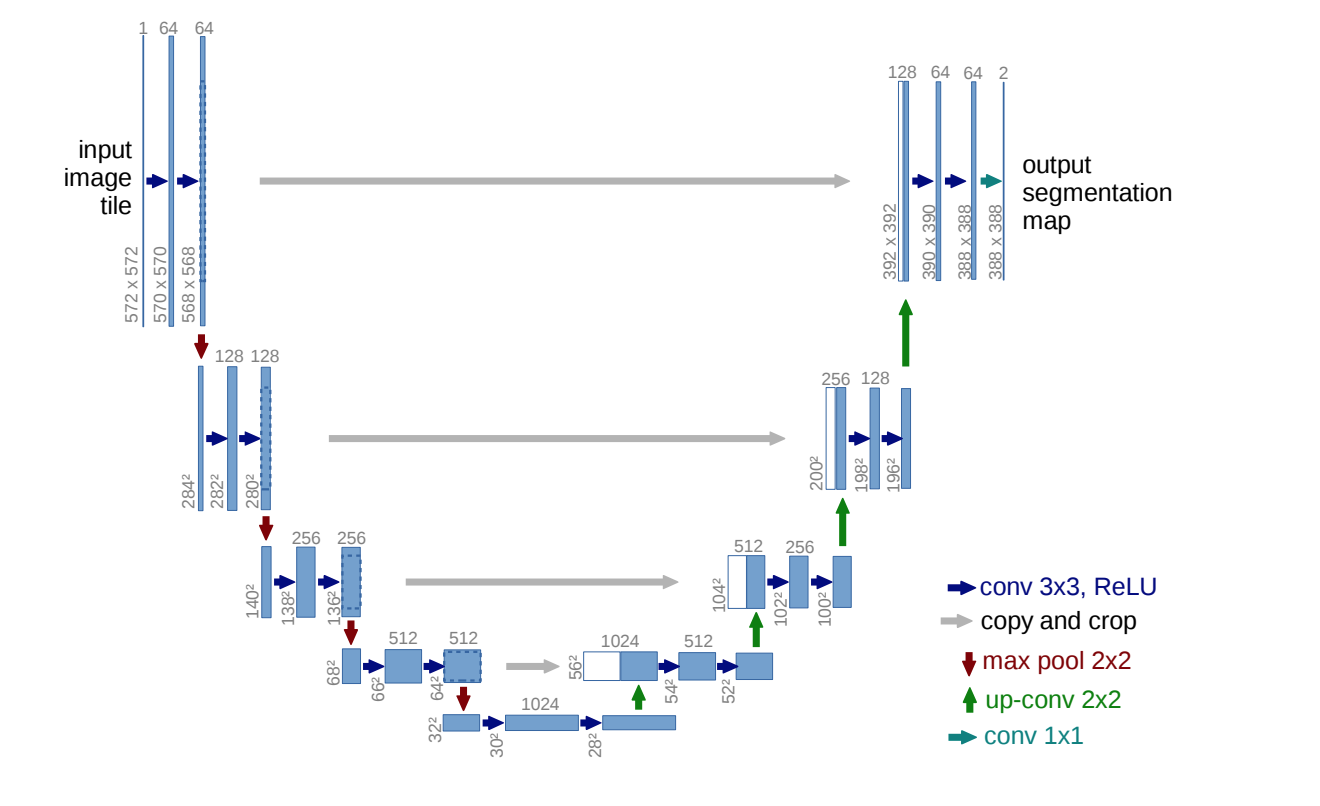
\includegraphics[width=10cm]{/home/thesis/images/UNet_Ronneberger.png}
    \caption{U-Net architecture, as illustrated in \cite{Ronneberger2015}. 
    Each blue box represents a multi-channel feature-map. 
    The number of channels is indicated above the box, the $x \times y$ dimensions are indicated at the bottom left.
    The gray arrows indicate the feature maps in the contracting path are copied and concatenated to the feature maps of the expanding path.}
    \label{fig:unet}
\end{SCfigure}


\subsubsection{Automated segmentation of the human spine}
\par{
    Multiple researchers have build systems for the automated segmentation of the human spine.
    Historically, this was done with techniques based on the calculation of mathematical and geometrical features of vertebrae. 
    For example in \cite{Klinder2008}, a model registration approach is used to segment a set of 10 \acrshort{ct} images.
    A parameteric geometrical model of a spine is optimized to fit the scan geometry as good as possible.
    These techniques showed to suffer from difficulties to generalize
    \footnote{Before the general introduction of deep learning, limits to the model's capability to generalize were observed in many different applications.
    This could be improved with deep learning networks, at the cost of requiring higher data volumes and often higher computation cost.}. 
    When the scan geometry does not match closely to an ideal spine, for example when a patient has severe scoliosis, this approach runs into problems.
}
\par{
    Deep learning models were developed for the problem \cite{Sekuboyina2017, Janssens, Chuang2019, Lessmann2018}.
    The model in \cite{Sekuboyina2017}\footnote{This model is developed on the xVertSeg dataset, which is one of the datasets used in this work. It is described starting on page \pageref{sec:xVertSeg}.} 
    uses a multi-step approach. First, the \acrfull{roi} (the lumbar region) is selected using a multilayer perceptron evaluated on the respones of a Canny Edge filter.
    This \acrshort{roi} is then sliced (sagittal) and crops ($270mm \times 270mm$\footnote{The article also mentions $27mm \times 27mm$, which seems to be a typo.}) are segmented with a 2D U-net. 
    The resulting masks are improved with a morphological closing filter. 
    In \cite{Janssens2018}, a similar 2 step approach is used. Here, the author chose to use a 3D U-net to evaluate patches from the \acrshort{roi} instead of a 2D U-net.
}
\par{
    An interesting approach to the problem is published in \cite{Lessmann2018, Chuang2019}. 
    The approach presented in this work makes used of the available prior anatomical knowledge of the human spine: 
    the vertebrae are located right next to each other and always occur in the same, known order.  
    The basis of the network in \cite{Lessmann2018} is an extended 3D U-Net, combined with an elaborate inference scheme.
    In \cite{Chuang2019}, this network was improved to reduce the memory required and the complexity of the inference scheme.
}
\par{
    In figure \ref{fig:lessmann_inference}, the inference scheme used in \cite{Lessmann2018} is illustrated.
    This is based on the anatomical knowledge that vertebrae occur in order, right next to each other.
    The network, illustrated in figure \ref{fig:chuang_architecture} in the version as presented in \cite{Chuang2019}, 
    performs instance segmentation of the scan by sequentially evaluating the model on 3-dimensional patches of the scan. 
    These patches have dimensions $180mm \times 180mm \times 180mm$ and can thus contain a full vertebra and meaningful parts of one or two adjacent vertebrae.
    The model is trained based on an image patch combined with a memory patch. This memory patch contains the voxels of the vertebrae that were already segmented in the sequential procedure.
    The network is trained to segment only the consecutive vertebra in sequence.
    For inference, the procedure starts by evaluating patches from the scan border until a (partial) vertebra is discovered and segmented.
    After storing this first segmented vertebra in the memory patch, the next vertebra is segmented from a patch that is centered on the previous vertebra and shifted down
    \footnote{The procedure works both for sampling up-down and down-up. Here, I stay with the procedure illustrated in figure \ref{fig:lessmann_inference}.}.
    Following this procedure, the vertebrae are segmented one by one.
    This procedure was developped on a collection of 103 medical images of the human spine, including the xVertSeg dataset (discussed on \pageref{sec:xVertSeg}). 
    To improve the segmentation result, a \textit{soft false positive} and \textit{soft false negative} loss is added to the cross entropy loss, where the voxels are weighted by the inverse of the distance to the segment border. 
    These terms increase the loss specifically for those voxels close to the edge of a vertebra.
}
\begin{SCfigure}[][htb]
    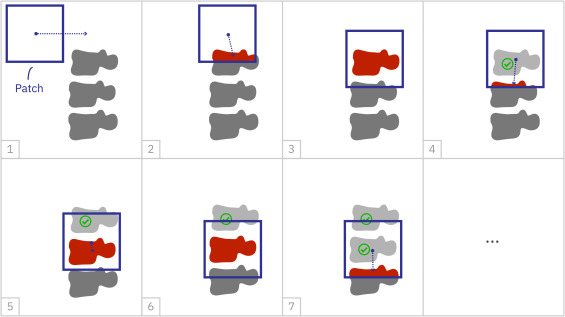
\includegraphics[width=10cm]{/home/thesis/images/Lessman_inference.jpg}
    \caption{Illustration of the inference scheme used in \cite{Lessmann2018} (image taken from same). }
    \label{fig:lessmann_inference}
\end{SCfigure}
\par{
    In \cite{Chuang2019}, some improvements to this procedure were introduced.
    The model is rendered less memory-intensive by passing the feature maps in the skip-connections after unpooling instead of directly.
    A method is developed to improve finding the starting point of the sequential segmentation procedure by evaluating only the patches where a high bone density is observed.
    The network is trained to output 3 values:
    \begin{description}
        \item[classification $C$]: A classification result of the segmented vertebra (in the specific evaluation step).
        \item[instance segmentation mask $S_1$]: A segmentation mask that is intended to output a segmentation mask that indicates to what vertebra instance every voxel in the patch belongs. 
        \item[Semantic segmentation mask $S_2$]: A binary segmentation mask that indicates whether a voxel belongs to a vertebra or to the background class.
    \end{description}
    To some extend, these three outputs seem redundant. 
    Since there is a very high geometric correlation between vertebrae, labelling the individual vertebrae is a very difficult task.
    Thus, a combination of different estimations is intended to procedure a more reliable labelling.
}
\begin{SCfigure}[][htb]
    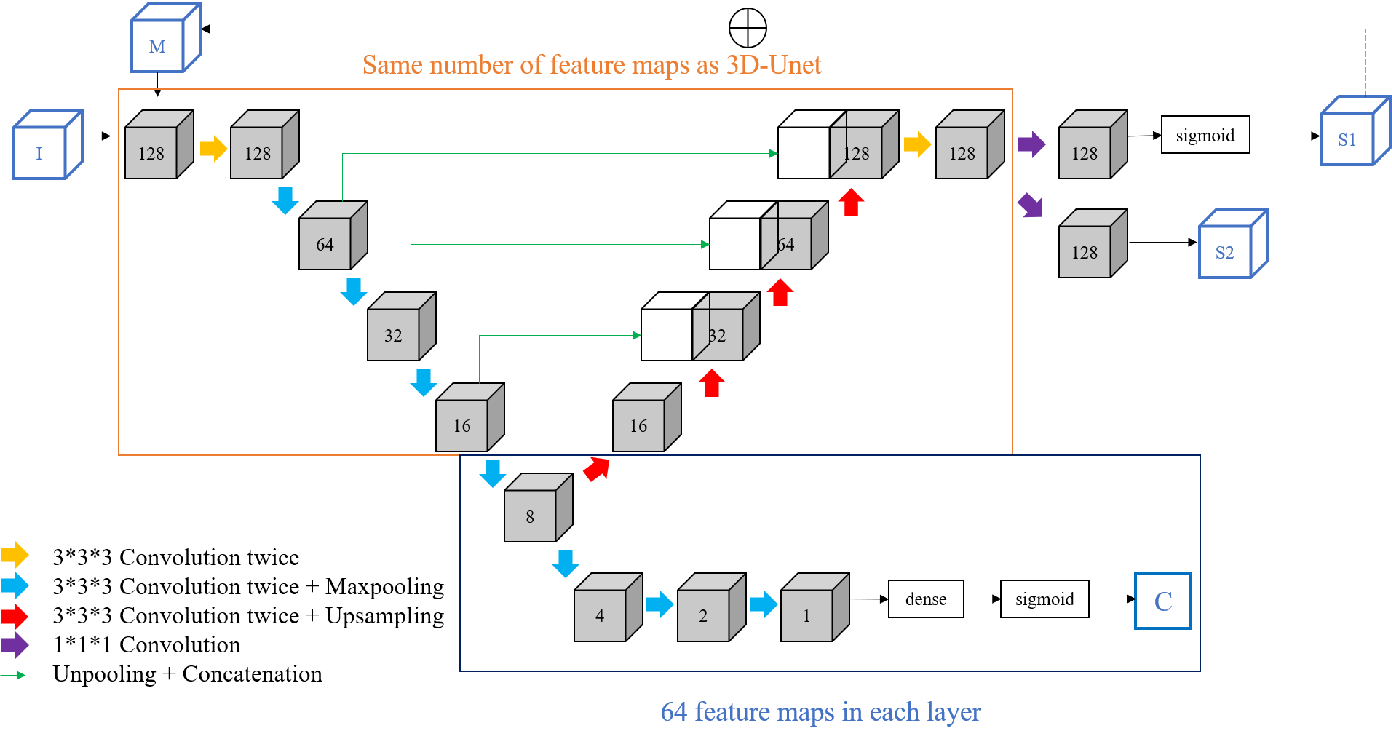
\includegraphics[width=10cm]{/home/thesis/images/Chuang_architecture.png}
    \caption{Extended U-Net architecture. Image from \cite{Chuang2019}.
    This network has }
    \label{fig:chuang_architecture}
\end{SCfigure}

%\todo[inline]{other authors, approaches --> priors used, metrics used, datasets used}


\section{Weakly supervised segmentation\label{sec:PreviousWork_weaklySupervised}}
\par{
    The subject of \Gls{weaklysupervisedl} is wide.
    Researchers devised a varied range of ideas to decrease the labelling cost by leveraging weak labels to infer strong results.
    Chapter \ref{sec:weak_supervision} discribes a number of different annotation types.
}
\subsection{Overview of different approaches}
\par{
    Given an image-level class label, the \Gls{caml} \todo{reference} allows to identify the picture regions responsible for a classification result \cite{Ahn2018, Ahn2019}
    \footnote{Other so-called \textit{saliency detection} methods exist, for example methods based on partial image occlusion [xxx].}.
    This is an approach that makes a lot of sense for example in cases where models are trained on web-scraped images.
    This approach is extended to the case of point-annotation in \cite{McEver2020}. 
    The rationale behind point annotation is that in cases where an expert is required to label the images, optimal use needs to be made of the expert's time.
    Based on estimations \cite{Bearman2015} the time consumption of point annotation and image level annotation is small, yet the information quality is higher (see also chapter \ref{sec:weak_supervision}).
    An expert does not need significantly more time to click on an object compared to providing an image label\footnote{
        It should be noted that point annotation refers to \textit{random} point annotation. Some authors \cite{Mainis} use \textit{extreme} point annotation. 
        Where the expert  is requested to indicate points at the edge of the segment region.
    }, yet the point provides valuable localization information.
    In \cite{McEver2020}, the case is even made that for large and dense images, point annotations could even help the expert to keep track of the already labelled objects.
    By using the annotation points, in a technique called \acrfull{pcam}, the authors of \cite{McEver2020} are able to improve the quality of the class affinity estimation compared to the regular \Gls{caml} technique (using the PASCAL VOC 2012 dataset).
    The obtained affinity maps are subsequently used as \textit{pseudo} label maps to train a network (ResNet50). 
    The author reports an improved performance of the model trained on \textit{pseudo} labels compared to the performance metric calculated for those pseudo labels.
}
\par{
    The technique to work in a two-step procedure, first estimating point guided pseudo-masks, then training a network based on these pseudo-masks is shared by different authors.
}
\subsection{Weakly supervised segmentation for Medical applications}
\par{
    The technique used in this project is inspired on the work of dr. I. Laradji in \cite{Laradji2020}.
    This researcher developed several methods to make use of weak supervised data for segmentation tasks.
    First, in \cite{Laradji2018}, the \Gls{wise} method is presented. 
    Contrary to other \Gls{weaklysupervisedl} projects, the authors focus on multi-class, multi-instace problems for which CAM-based solutions are less suitable.
    This method, illustrated in figure \ref{fig:Laradji_WISE}, consists of two branches from the same backbone: the Embedding branch and the Localization branch.
    The Embedding branch is trained with a pre-trained class-agnostic object proposal method. 
    This network (FCN8) is pre-trained to output similar embeddings for pixels that belong to the same class.
    The output of the network is thus an Embedding mask for each pixel of the image. 
    This network is trained to deliver different embeddings for different object instances with a binary binary cross entropy function on the squared exponential kernel difference of the embeddings
    \footnote{With $E_i$ and $E_j$ the embeddings for points $i$ and $j$ and $\mathcal{I}$ the collection of labelled points.}:
}
\begin{eqnarray}
    S(i,j) &=& \exp \left( \frac{||E_i-E_j||^2}{2d} \right)\\
    \mathcal{L}_E &=& - \sum_{(i,j)\in \mathcal{I}} \left[  \mathbf{I}(y_i=y_j) log(S(i,j)) + \mathbf{I}(y_i\neq y_j) log(1-S(i,j))  \right]
\end{eqnarray}
\par{
    The second part of the \Gls{wise} network is the Localization branch. 
    This branch aims to predict small \textit{blobs} at the center of each object.
    These blobs are too small to serve as masks on their own, but they can be combined with the E-branch result to provide segmentation masks.
}
\begin{SCfigure}[][htb]
    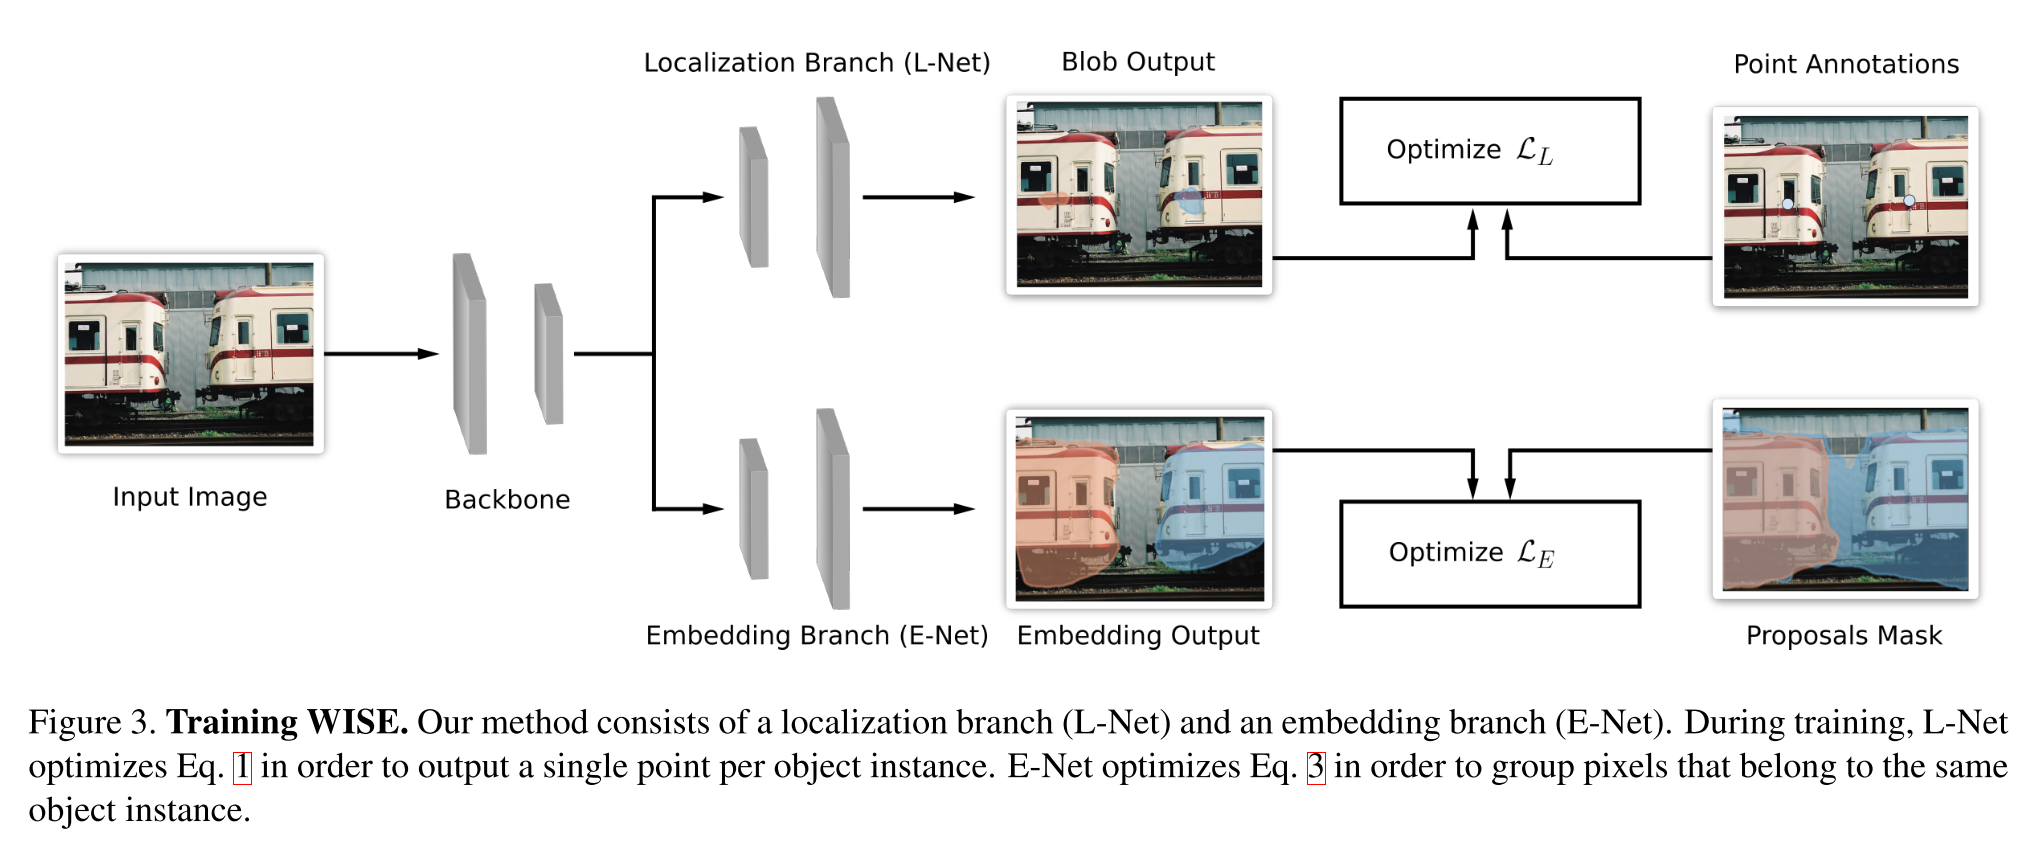
\includegraphics[width=10cm]{/home/thesis/images/Laradji_architecture.png}
    \caption{Illustration from \cite{Laradji2020}. The \Gls{wise} approach consists of two branches: The Embedding branch and the Localization branch.}
    \label{fig:Laradji_WISE}
\end{SCfigure}
\par{
    The \Gls{wise} model seems to perform well on the PASCAL VOC 2012 dataset, the Cityscapes dataset and the COCO 2014 dataset. 
    Nevertheless, the author abandoned it in \cite{Laradji2020}, where he demonstrated a weakly supervised network to segment patient lungs and zones of opacity and consolidation in the lungs of potential \Gls{covid} patients.
    There are several potential reasons for this. 
    Two of those seem important for this work. 
    First, the \Gls{wise} approach seems to assume the expert positions the annotation point right in the center of each object instance.
    Second, the approach is complex and the double branch inference is computation and memory intensive. 
    In this project, it is assumed that experts can provide different point labels for the same instance at random locations in the instance.
    Since volume data is is more memory intensive than picture data, it is beneficial to avoid overly complex and memory intensive approaches.
}
\par{
    In \cite{Laradji2020}, Laradji et al. introduces an approach based on the consistency loss, combined with binary cross entropy.
    This approach is used and extended in this project.
    Details are provided starting on page \pageref{sec:model_concept}.
}